\chapter{Breve Descrição do Projeto de Formatura}

O projeto de formatura tem como objetivo o desenvolvimento de um sistema de automação residencial completo, com foco na robustez, segurança e facilidade de uso. Para tanto, a modelagem de uma arquitetura flexível, mas que suportasse os requisitos iniciais, tem papel essencial no trabalho. A plataforma do sistema é enfática em sua proposta de camadas, na qual a integração entre os níveis é feita por meio de troca de mensagens, utilizando a infraestrutura de comunicação desenvolvida. A \autoref{fig:sistemaHedwig} ilustra o sistema como um todo.

\begin{figure}[H]
	\caption{\label{fig:sistemaHedwig}Sistema Hedwig}
	\begin{center}
		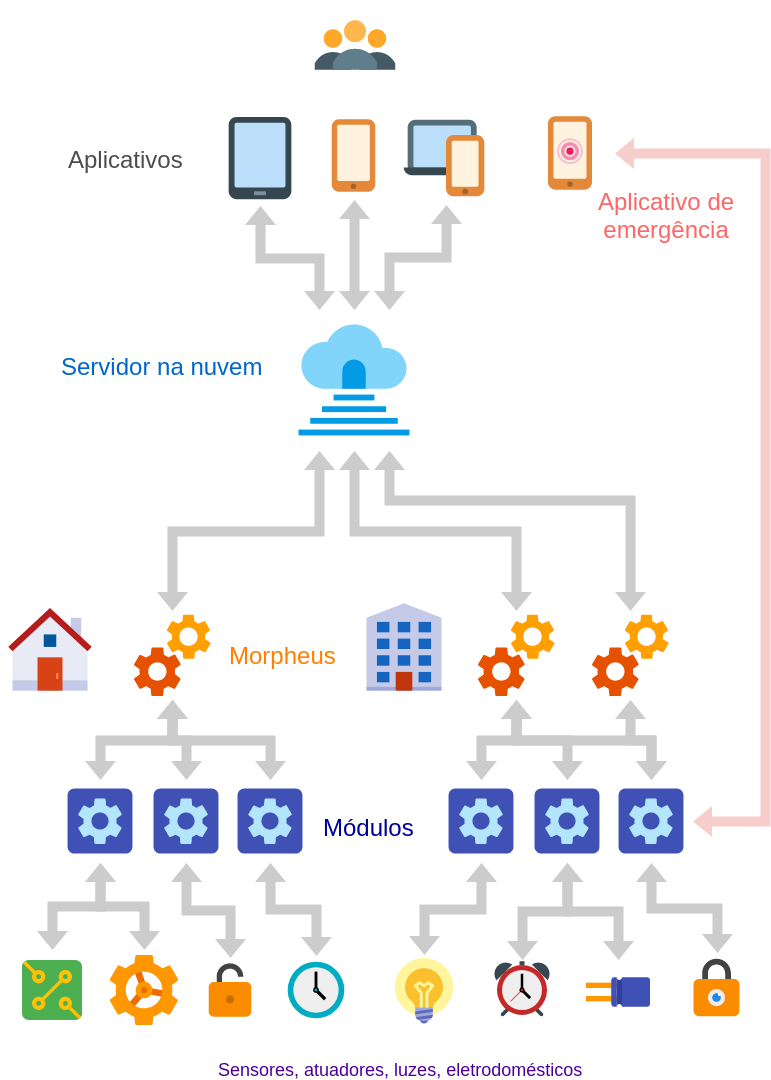
\includegraphics[width=0.8\textwidth]{sistemaHedwig}
	\end{center}
	\legend{Fonte: os autores}
\end{figure}

No decorrer desta seção, serão apresentados os pontos essenciais do projeto, bem como a descrição das soluções adotadas.

\section{Hardware}

Para a criação dos módulos de hardware, foram escolhidos componentes de \wiot{} comerciais, que possuem preços acessíveis, ampla documentação disponível e uma comunidade de desenvolvedores crescente.

A interconexão dos componentes, bem como a comunicação com o mundo externo pela internet será intermediada por um servidor local, que rodará na plataforma Raspberry Pi, rodando um sistema operacional Linux (Raspbian, baseado em Debian) e que dispõe da interface de hardware necessária para conexão com a rede.

Os sensores e atuadores devem ser conectados fisicamente com um módulo controlador, de modo que, para contornarmos essa limitação, utilizaremos módulos ESP8266 para transmissão sem fio por meio de Wi-Fi. Esses módulos serão responsáveis pela transmissão das informações recebidas para o servidor local. 

\begin{figure}[H]
	\caption{\label{fig:QuatroModulos}Módulos de Hardware}
	\begin{center}
		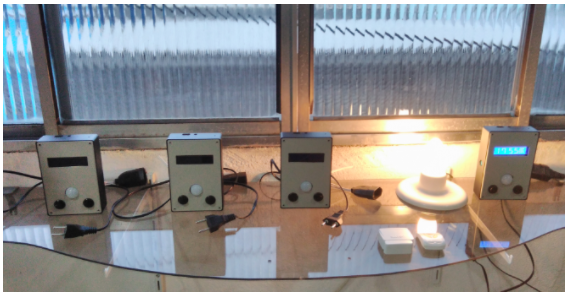
\includegraphics[scale=0.5]{QuatroModulos}
	\end{center}
	\legend{Fonte: os autores}
\end{figure}

Em geral, esses módulos consistem do microcontrolador, relés, sensores e fontes/conversores de tensão a depender do módulo, além de um circuito para manutenção corretiva baseado no astável 555, conectados à rede Wi-Fi e/ou trabalhando como pontos de acesso. Para casos de falha de conexão, há um algoritmo de novas tentativas com tempos progressivamente maiores conforme as falhas ocorrerem, que busca deixar o módulo disponível para outras funções enquanto o serviço não está disponível. Para evitar o travamento, um sinal de \textit{keep alive} é monitorado, e um circuito anti-travamento deve ativar um \textit{hard reset} (reset por hardware), ou então uma rotina de \textit{soft reset} é acionada.

\begin{figure}[H]
	\caption{\label{fig:diagramaModuloBase}Diagrama do Módulo de Iluminação}
	\begin{center}
		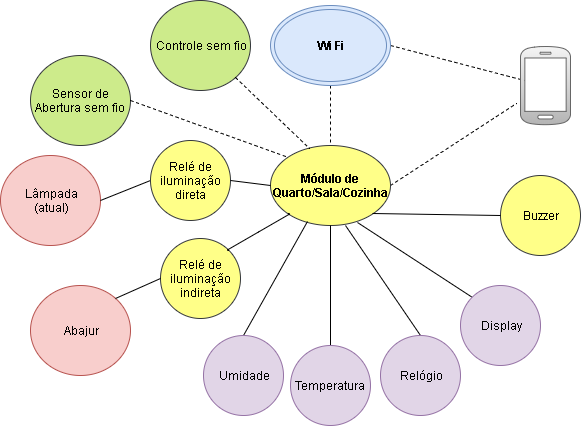
\includegraphics[scale=0.5]{diagramaModuloBase}
	\end{center}
	\legend{Fonte: os autores}
\end{figure}


\section{Software}

As partes de software do sistema são divididas de acordo com a sua aplicação, localização e uso.

Em contato mais próximo dos dispositivos de hardware está o servidor local, Morpheus. O servidor local é responsável pela interconexão dos módulos da casa com os serviços de nuvem disponíveis. A troca de informação entre os módulos físicos e o Morpheus é realizada por meio de mensagens, codificadas em um protocolo desenvolvido pelo grupo, e encaminhadas por meio do protocolo MQTT, com um broker local disponível na residência. O envio de mensagens é feito em tópicos, aos quais o módulo pode publicar ou se inscrever de acordo com o seu serial number, de modo a evitar que um módulo consiga ter acesso ao canal de outro módulo. O servidor local, no entanto, precisa de um certificado válido para que possa se inscrever no seu canal, onde a troca de mensagens é realizada com criptografia assíncrona. Quando a mensagem chega nesse servidor, ela é convertida em um formato intermediário e colocada em um fila de entrada, onde uma thread de um pool irá retirá-la para efetuar o processamento, e conversão para um JSON esperado pela nuvem.

A segunda transmissão de dados, entre o Morpheus e os serviços de nuvem é feita por meio de um canal WebSocket, no qual a conexão permanece ativa a todo o momento. Os serviços de nuvem tratam a chegada da mensagem, e interagem com um cliente web, por meio de um dashboard, sobre o qual o usuário pode interagir.

\begin{figure}[htb]
	\caption{\label{fig:dashboard}Dashboard}
	\begin{center}
		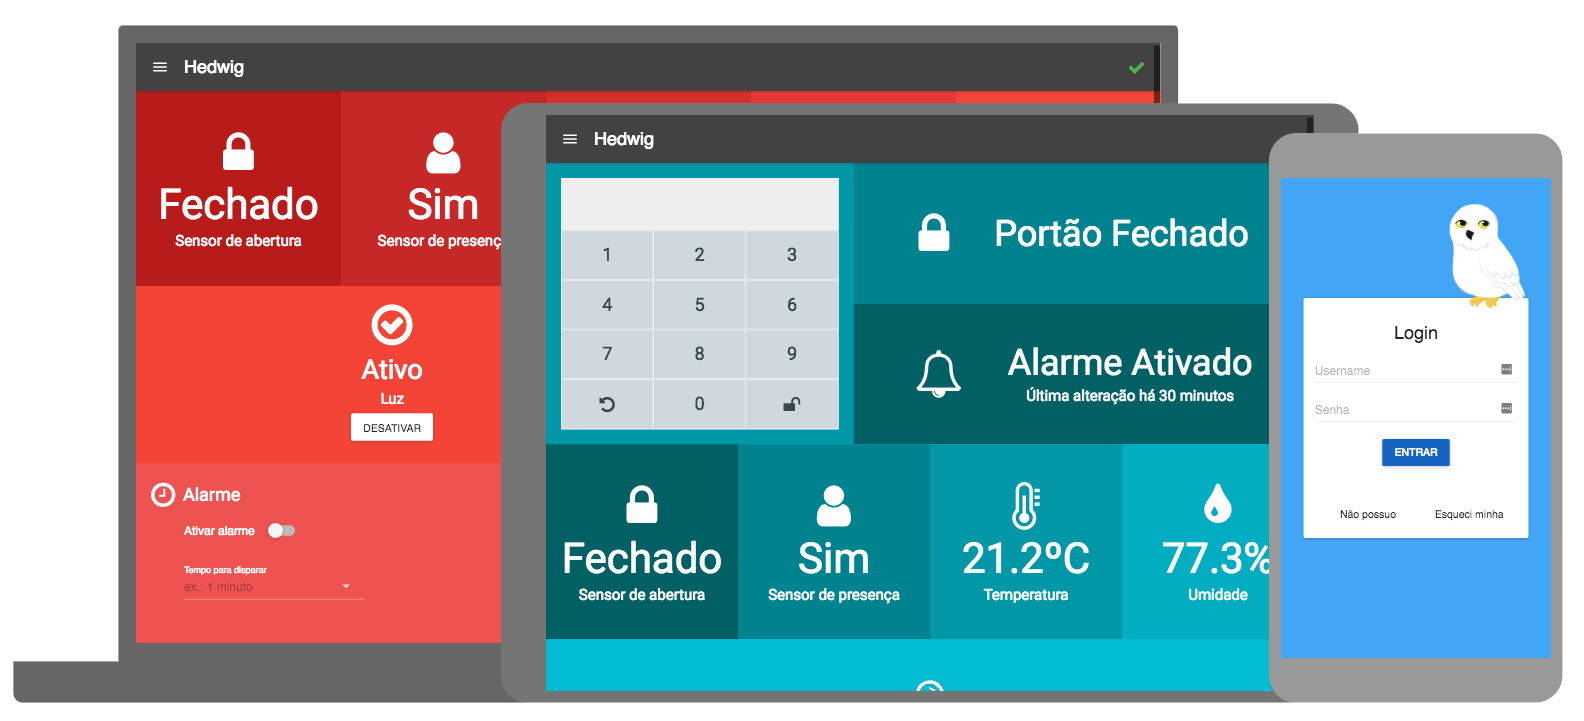
\includegraphics[width=0.8\textwidth]{dashboard}
	\end{center}
	\legend{Fonte: os autores}
\end{figure}

Para que a robustez do sistema seja assegurada, o projeto também conta com um sistema emergencial, no caso de não haver internet na casa ou de ocorrer qualquer problema com o servidor local. O usuário pode se conectar diretamente na rede de um dos módulos, sem a integração com a nuvem, utilizando um aplicativo de backup.

\section{Bases de Dados}

São usadas duas bases de dados na implementação do Hedwig. O primeiro é um banco de dados não-relacional baseado em documentos, que armazena dados coletados pelos sensores e informações sobre as entidades relevantes ao sistema - usuários e seus dispositivos conectados. O segundo é um banco de dados em memória que guarda informações sobre os dispositivos que estão conectados à nuvem no momento, facilitando a comunicação entre aplicativos e os controladores de cada casa.

\begin{figure}[H]
	\caption{\label{fig:Cloud}Arquitetura da Nuvem}
	\begin{center}
		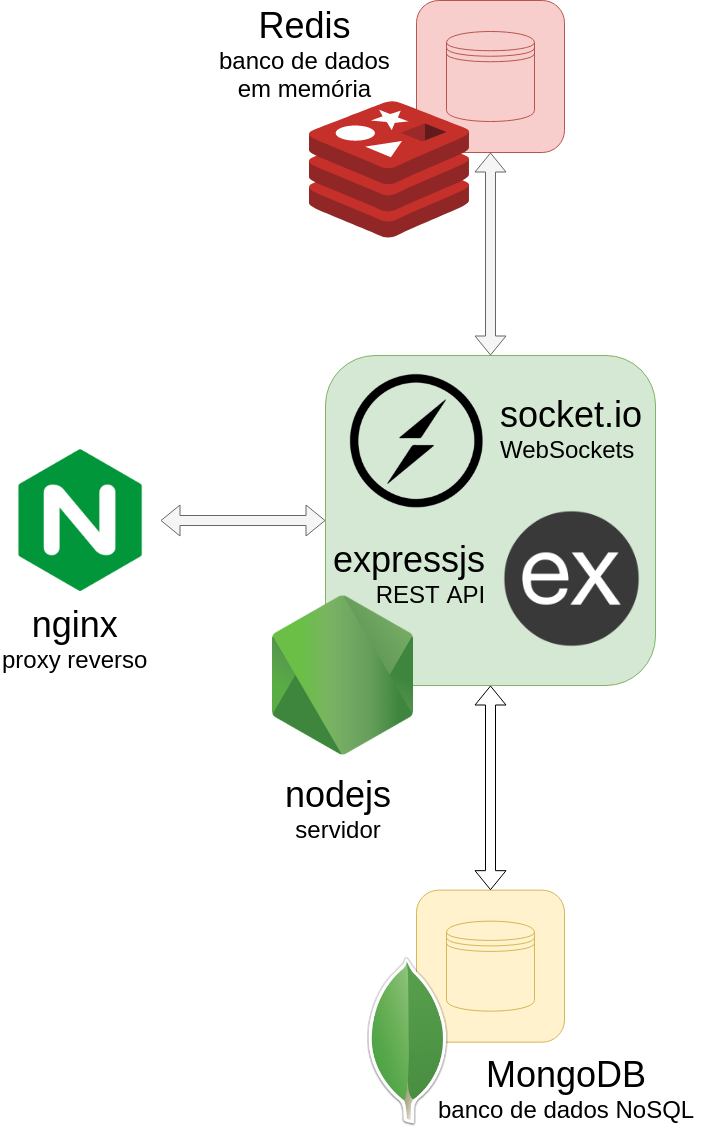
\includegraphics[width=0.6\textwidth]{Cloud}
	\end{center}
	\legend{Fonte: os autores}
\end{figure}

\subsection{Dados de Sensores, Dispositivos e Usuários}

É usado o MongoDB como banco de dados principal. O MongoDB é um banco de dados não-relacional, gratuito e \emph{open-source} baseado em documentos, que são representados como objetos com pares chave-valor similares aos objetos JSON. Essa escolha deve-se ao fato de que o maior volume de dados armazenados são os valores dos sensores, que podem ser facilmente modelados como documentos. Outros fatores que influenciaram a escolha do MongoDB foram sua escalabilidade, que pode ser realizada por replicação ou "clustering", e a flexibilidade de poder implementar facilmente mudanças nas propriedades das entidades.

\subsection{Dados de Conexões Ativas}

Para facilitar o encaminhamento de dados --- tanto informações coletadas pelos sensores como comandos de ação e configuração --- entre controladores locais e aplicativos cliente, foi usado o Redis, um banco de dados em memória capaz de armazenar estruturas como strings, listas, hashes, conjuntos ordenados e não-ordenados, indíces de geolocalização, entre outros. Devido à sua performance, o Redis é frequentemente usado para cache de páginas, aplicações de mensageria, implementação de filas e armazenamento de dados de sessão. No caso do Hedwig, ele é usado para esta última aplicação, guardando dados dos controladores e aplicativos conectados à nuvem no momento.

\section{Redes e Conectividade}

A conectividade local, planejada sobre a infraestrutura de comunicação disponível, é feita por meio de ondas de rádio, na frequência comercial relativa às redes Wi-Fi. Cada um dos módulos possui um microcontrolador e radiotransmissor ESP8266, o qual se conecta à rede da residência e envia mensagens para o respectivo tópico. Os módulos possuem tópicos específicos, cujos nomes são finalizados em "m2s" (\emph{module to server}) e contêm o serial ID do módulo em questão. Essa garantia é feita por meio de configurações no broker, no qual assegura-se dr que o endereço do tópico possui as credenciais do módulo autenticado.

O servidor local possui um tópico específico, cujo nome é finalizado em "s2m" (\emph{server to module}), e tem acesso de subscrição a todos os tópicos relativos às publicações de módulos. A autenticação do servidor, ao contrário daquela dos módulos, é feito por meio de certificados digitais, e há criptografia assíncrona na camada de transporte (SSL).

Para a comunicação entre a casa e a nuvem, ocorreram mudanças durante o planejamento da arquitetura. De início, o projeto estabelecia que o servidor local também tivesse a responsabilidade de ser um servidor para requisições externas, oferecendo para isso uma API REST. Entretanto, os impactos dessa decisão afetam criticamente a segurança, já que a casa estaria suscetível a ataques de negação de serviço (DoS). Assim, posteriormente, optou-se pela utilização de WebSockets na implementação dessa comunicação, de modo que a conexão entre controlador local e nuvem permanece ativa, e a responsabilidade por se proteger de ataque do tipo concentra-se nesta última, onde há uma infraestrutura muito mais robusta e existe possibilidade de uso de serviços de terceiros, como servidores Akamai.

Em alto nível, é representado na \autoref{fig:arquiteturaHedwig} o diagrama arquitetural do projeto. Na \autoref{fig:diagramaDeComunicacao}, é disponibilizada a arquitetura do servidor local (Morpheus) e a sua conectividade com a nuvem e módulos.

\begin{figure}[H]
	\caption{\label{fig:arquiteturaHedwig}Diagrama Arquitetural}
	\begin{center}
	    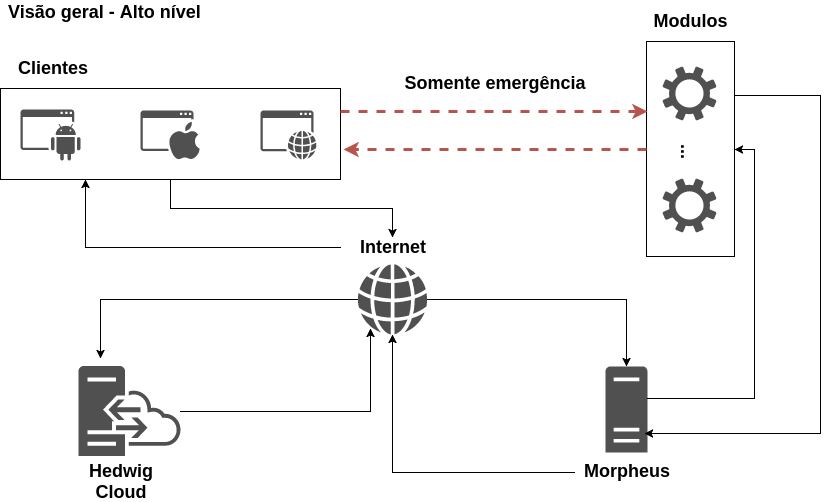
\includegraphics[width=0.9\textwidth]{arquiteturaHedwig}
	\end{center}
	\legend{Fonte: os autores}
\end{figure}

\begin{figure}[H]
	\caption{\label{fig:diagramaDeComunicacao}Diagrama de Comunicação}
	\begin{center}
	    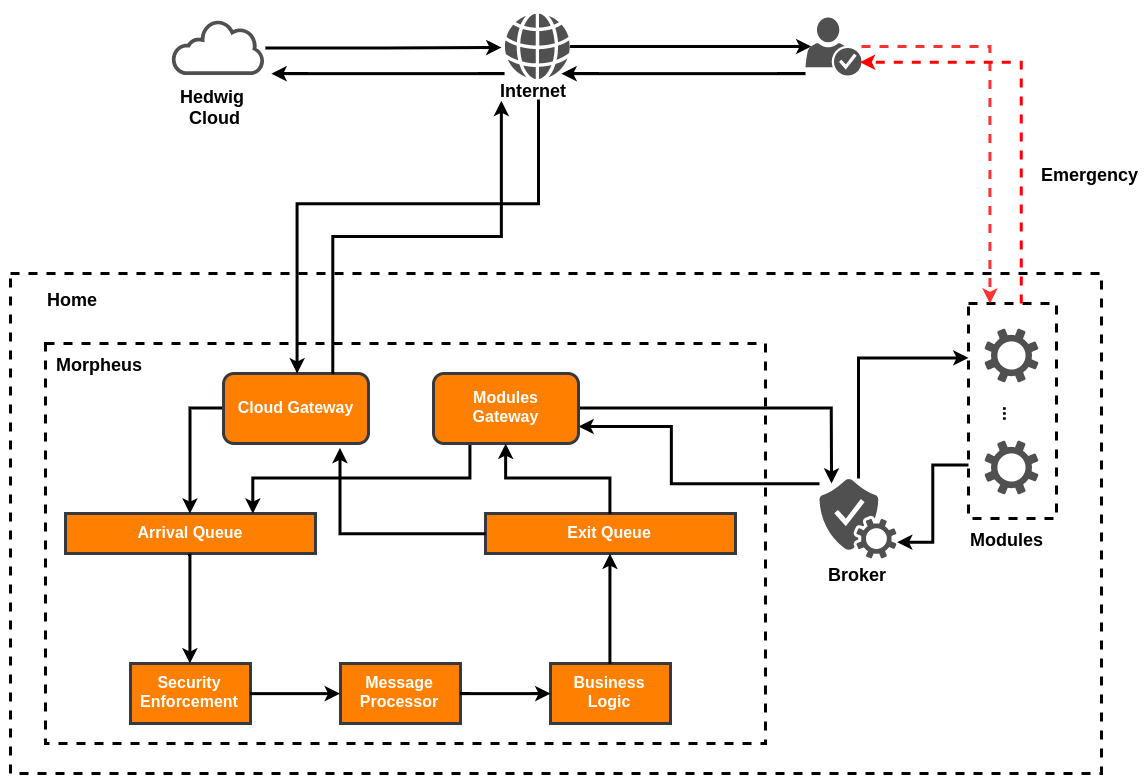
\includegraphics[width=0.9\textwidth]{diagramaDeComunicacao}
	\end{center}
	\legend{Fonte: os autores}
\end{figure}

% TODO diagrama de interação
